\documentclass[a4paper,10pt]{article}

\usepackage[utf8]{inputenc}
\usepackage{amssymb,amsmath}
\usepackage{pbox}
\usepackage[margin=1in]{geometry}
\usepackage{xr}
\usepackage{pdflscape}
\usepackage{graphicx}
\usepackage{verbatim}

%opening
\title{Review Information}

\begin{document}

\date{}
\maketitle
\tableofcontents

\newpage
\section{Comparison of \textit{k}-mer Sizes}

We perform similar experiments as in the main text to investigate the consequences of using \textit{k}-mer sizes similar to those used in sequence assembly instead of Neptune's automatically calculate \textit{k}-mer sizes. We present the results of our comparisons in Tables \ref{table:insilico_kmers}, \ref{table:4bv12a_kmers}, and \ref{table:ecoli_kmers}.

As the signatures are consolidated from multiple inclusion targets, rather than using a single reference genome from which to extract signatures, it is possible for signatures to overlap each other. Additionally, the reported lengths are with respect to the signature FASTA record, whereas the coordinates are with respect to a BLAST alignment to the reference genome. As such, it is possible for the reported signature lengths and signature coordinates to be slightly different from each other.

\subsection{Simulated Dataset}

This section corresponds to the first experiment performed in the main text using an artificial \textit{B. anthracis}-\textit{V. cholerae} dataset. We compare the consequence of using \textit{k}-mer sizes used in sequence assembly instead of Neptune's automatically calculated \textit{k}-mer sizes. There are six signatures of known length and location inserted into our artificial inclusion genome. We compare top-scoring (\(\geq\) 0.95) signatures identified when using Neptune's calculated \textit{k}-mer size of 27 against \textit{k}-mer sizes 19 and 21. The results of this comparison are presented in Table \ref{table:insilico_kmers}.

\subsubsection*{\textit{k} = 27}

The following command line arguments (with truncated directory locations) were used to run the artificial \textit{B. anthracis}-\textit{V. cholerae} \textit{k} = 27 experiment:

\begin{verbatim}
neptune
--kmer 27
--inclusion insilico/inclusion/
--exclusion insilico/exclusion/
--organization 3 --exhits 2
--drmaa --default-specification "-l h_vmem=10G -pe smp 4"
--output insilico/insilico-neptune/
\end{verbatim}

\subsubsection*{\textit{k} = 19}

The following command line arguments (with truncated directory locations) were used to run the artificial \textit{B. anthracis}-\textit{V. cholerae} \textit{k} = 19 experiment:

\begin{verbatim}
neptune
--kmer 19
--inclusion insilico/inclusion/
--exclusion insilico/exclusion/
--organization 3 --exhits 2
--drmaa --default-specification "-n 1 --nodes=1 --ntasks-per-node=1 --mem=10240"
--output insilico_k19/
\end{verbatim}

\subsubsection*{\textit{k} = 21}

The following command line arguments (with truncated directory locations) were used to run the artificial \textit{B. anthracis}-\textit{V. cholerae} \textit{k} = 21 experiment:

\begin{verbatim}
neptune
--kmer 21
--inclusion insilico/inclusion/
--exclusion insilico/exclusion/
--organization 3 --exhits 2
--drmaa --default-specification "-n 1 --nodes=1 --ntasks-per-node=1 --mem=10240"
--output insilico_k21/
\end{verbatim}

\begin{landscape}
\mbox{}\vfill
\begin{table}[!h]
\renewcommand{\arraystretch}{1.2}
\centering
\begin{tabular}{| c | c c | c c c | c c c | c c c |}
  \cline{1-12}
  & \multicolumn{2}{c|}{\textbf{Actual}} & \multicolumn{3}{c|}{\textbf{k = 27}} & \multicolumn{3}{c|}{\textbf{k = 19}} & \multicolumn{3}{c|}{\textbf{k = 21}} \\
  \cline{2-4} \cline{4-6} \cline{7-9} \cline{10-12}
  \textbf{Number} & \textbf{Length} & \textbf{Coordinates} & \textbf{Score} & \textbf{Length} & \textbf{Coordinates} & \textbf{Score} & \textbf{Length} & \textbf{Coordinates} & \textbf{Score} & \textbf{Length} & \textbf{Coordinates} \\ \cline{1-12}
  1 & 23338 & 757541 - 780879 & 0.98 & 23324 & 757468 - 780791 & 0.98 & 548 & 757476 - 758020 & 0.98 & 23330 & 757462 - 780791 \\
  & & & & & & 0.98 & 22091 & 758044 - 780130 & & & \\
  & & & & & & 0.99 & 638 & 780154 - 780791 & & & \\ \cline{1-12}
  2 & 50038 & 1538334 - 1588372 & 0.98 & 10136 & 1538248 - 1548380 & 0.98 & 9807 & 1538248 - 1548054 & 0.98 & 50038 & 1538248 - 1588285 \\
  & & & 0.98 & 39763 & 1548525 - 1588285 & 0.98 & 21448 & 1541070 - 1562520 & & & \\
  & & & & & & 0.98 & 6477 & 1562540 - 1569016 & & & \\
  & & & & & & 0.98 & 16603 & 1569035 - 1585639 & & & \\
  & & & & & & 0.98 & 7327 & 1580959 - 1588285 & & & \\ \cline{1-12}
  3 & 12259 & 2345827 - 2358086 & 0.98 & 12248 & 2345741 - 2357988 & 0.98 & 8394 & 2345741 - 2354516 & 0.98 & 12254 & 2345741 - 2357994 \\
  & & & & & & 0.98 & 3798 & 2354199 - 2357996 & & & \\ \cline{1-12}
  4 & 9652 & 3115541 - 3125193 & 0.98 & 9643 & 3115463 - 3125105 & 0.98 & 9650 & 3115456 - 3125105 & 0.98 & 9649 & 3115457 - 3125105 \\ \cline{1-12}
  5 & 4282 & 2882648 - 3886930 & 0.98 & 4280 & 3882564 - 3886843 & 0.96 & 829 & 3882562 - 3883390 & 0.98 & 4282 & 3882562 - 3886843 \\
  & & & & & & 0.98 & 3398 & 3883446 - 3886843 & & & \\ \cline{1-12}
  6 & 10155 & 4644385 - 4654540 & 0.98 & 10154 & 4644299 - 4654452 & 0.98 & 729 & 4644318 - 4645045 & 0.98 & 10154 & 4644299 - 4654452 \\
  & & & & & & 0.98 & 9384 & 4645069 - 4654452 & & & \\ \cline{1-12}
\end{tabular}%
\caption{A comparison of top-scoring (\(\geq\) 0.95) identified signatures when using Neptune's calculated \textit{k}-mer size (\textit{k} = 27) against common \textit{k}-mer sizes used in assembly (\textit{k} = 19, 21). The data is an artificial \textit{B. anthracis}-\textit{V. cholerae} genome dataset. The coordinates are taken from a BLAST reference mapping and the lengths are taken from the actual signature length.}
\label{table:insilico_kmers}
\end{table}
\vfill
\end{landscape}

\subsubsection*{Observations}

We observe that the signatures produced for Neptune's automatically calculated \textit{k}-mer size (\textit{k} = 27) and \textit{k} = 21 are very similar. One notable difference is signature \#2 is reported as two adjacent signatures when \textit{k} = 27 and is reported as a single signature when \textit{k} = 21. However, although \textit{k} = 19 reports the same regions as signatures as \textit{k} = 21 and \textit{k} = 27, many more of these signatures are reported as adjacent and even overlapping signatures. Nonetheless, the signatures identified when using all three \textit{k}-mer sizes agree about the regions of the genome that correspond to signature sequence (Figure \ref{figure:insilico_kmers}).

\begin{figure}
\centering
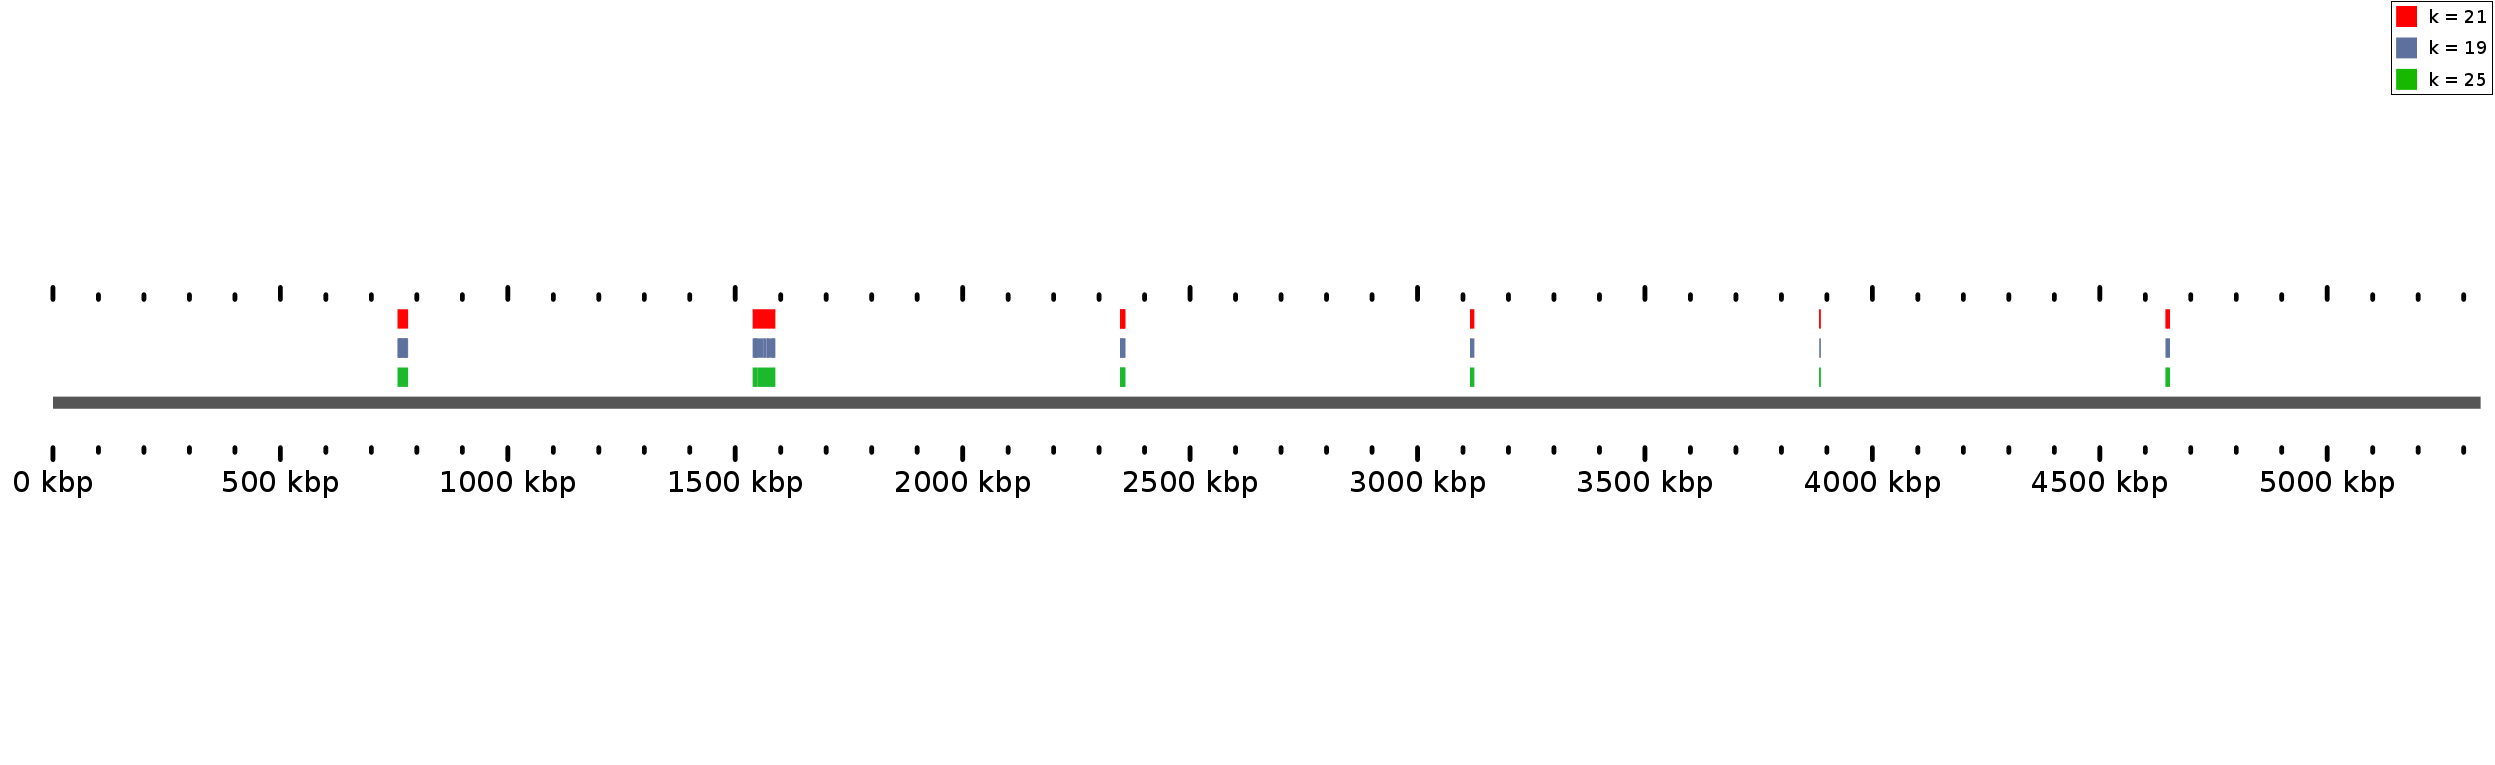
\includegraphics[width=1.0\textwidth]{insilico_kmers_crop.png}
\caption{A high-level visualization of the signatures identified by Neptune using \textit{k}-mers of different sizes when run on an artificial \textit{B. anthracis}-\textit{V. cholerae} genome data set. There is considerable agreement about the regions of the genome corresponding to signature sequence.}
\label{figure:insilico_kmers}
\end{figure}

\subsection{Listeria monocytogenes}

This section corresponds to the second group of experiments performed in the main text using a \textit{Listeria monocytogenes} serotype 1/2a and serotype 4b dataset. We compare the consequence of using \textit{k}-mer sizes used in sequence assembly instead of Neptune's automatically calculated \textit{k}-mer sizes. We compare Neptune's top-scoring (\(\geq\) 0.95) signatures when automatically calculateing a \textit{k}-mer size of 25 against \textit{k}-mer sizes 19 and 21, using the signatures identified when \textit{k} = 25 as the basis of the comparison. The results of the 4b inclusion and 1/2a exclusion experiment are presented in Table \ref{table:4bv12a_kmers}.

\subsubsection*{\textit{k} = 25}

The following command line arguments (with truncated directory locations) were used to run the \textit{L. monocytogenes} 4b inclusion and 1/2a exclusion experiment with \textit{k} = 25:

\begin{verbatim}
neptune
--kmer 25
--inclusion listeria/training/4b/
--exclusion listeria/training/1-2a/
--organization 3 --exhits 2 --seed-size 5
--drmaa --default-specification "-l h_vmem=10G -pe smp 4"
--output listeria/listeria-neptune-4b/
\end{verbatim}

\subsubsection*{\textit{k} = 19}

The following command line arguments (with truncated directory locations) were used to run the \textit{L. monocytogenes} 4b inclusion and 1/2a exclusion experiment with \textit{k} = 19:

\begin{verbatim}
neptune
--kmer 19
--inclusion listeria/training/4b/
--exclusion listeria/training/1-2a/
--organization 3 --exhits 2 --seed-size 5
--drmaa --default-specification "-n 1 --nodes=1 --ntasks-per-node=1 --mem=10240"
--output listeria4b_k19
\end{verbatim}

\subsubsection*{\textit{k} = 21}

The following command line arguments (with truncated directory locations) were used to run the \textit{L. monocytogenes} 4b inclusion and 1/2a exclusion experiment with \textit{k} = 21:

\begin{verbatim}
neptune
--kmer 21
--inclusion listeria/training/4b/
--exclusion listeria/training/1-2a/
--organization 3 --exhits 2 --seed-size 5
--drmaa --default-specification "-n 1 --nodes=1 --ntasks-per-node=1 --mem=10240"
--output listeria4b_k21
\end{verbatim}

\subsubsection*{Observations}

The signatures identified by Neptune for all three \textit{k}-mer lengths (\textit{k} = 19, 21, 25) are generally in agreement, with shorter \textit{k}-mers (\textit{k} = 19) more frequently being split into several smaller adjacent signatures, rather than being reported as a single contiguous signature. This is also observed for signature \#3 when \textit{k} = 21. However, as this experiment is performed with real data, it is difficult to assess what the true signature lengths should be in this circumstance. Nonetheless, we might infer from the results of the simulated dataset experiment (above) that when \textit{k} = 19, signatures are being split into adjacent signatures more frequently than they should be.

\begin{figure}
\centering
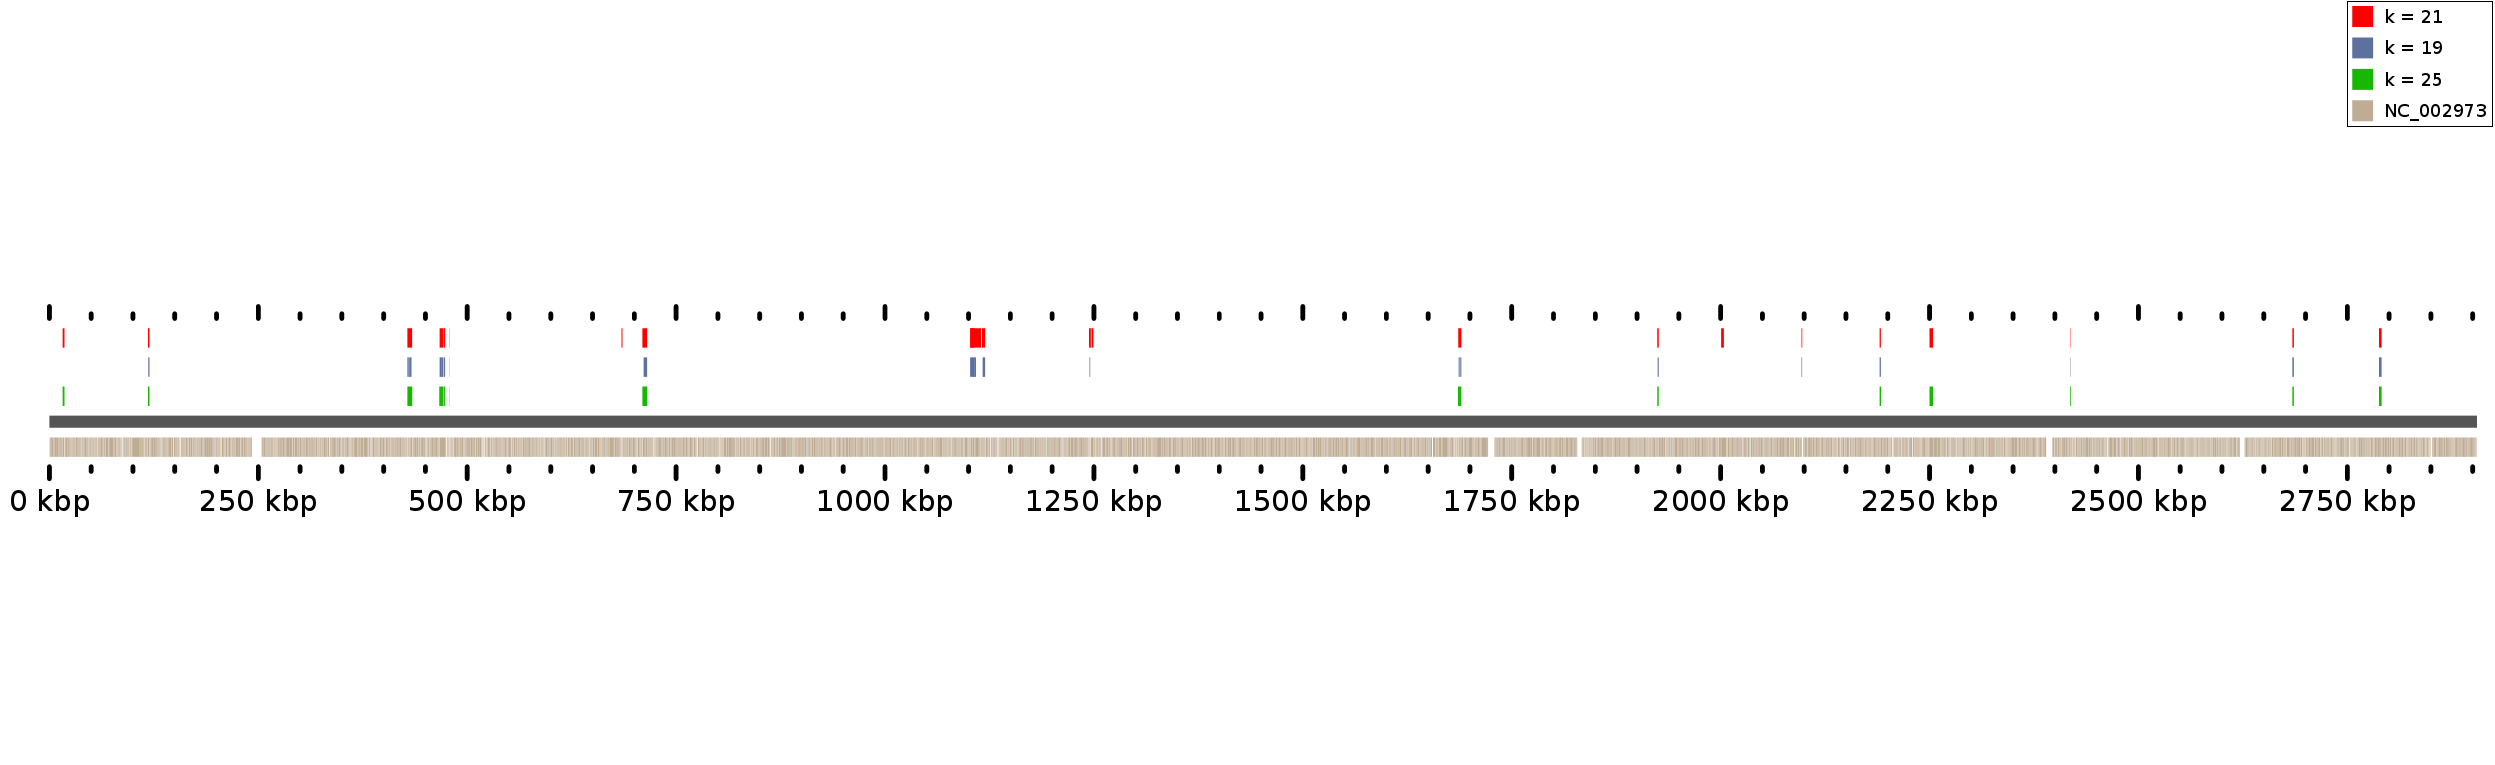
\includegraphics[width=1.0\textwidth]{listeria4b_kmers_crop.png}
\caption{A high-level visualization of the signatures identified by Neptune using \textit{k}-mers of different sizes when run on a \textit{L. monocytogenes} serotype 4b inclusion and serotype 1/2a exclusion data set. In general, there is agreement about the regions of the genome corresponding to signature sequence.}
\label{figure:listeria4b_kmers}
\end{figure}

\begin{landscape}
\mbox{}\vfill
\begin{table}[!h]
\renewcommand{\arraystretch}{1.2}
\centering
\begin{tabular}{| c | c c c | c c c | c c c |}
  \cline{1-10}
  & \multicolumn{3}{c|}{\textbf{k = 25}} & \multicolumn{3}{c|}{\textbf{k = 19}} & \multicolumn{3}{c|}{\textbf{k = 21}} \\
  \cline{2-4} \cline{5-7} \cline{8-10}
  \textbf{Rank} & \textbf{Score} & \textbf{Length} & \textbf{Coordinates} & \textbf{Score} & \textbf{Length} & \textbf{Coordinates} & \textbf{Score} & \textbf{Length} & \textbf{Coordinates} \\ \cline{1-10}
  1 & 0.99 & 223 & 478246 - 478468 & 0.97 & 341 & 478135 - 478474 & 0.99 & 231 & 478242 - 478472 \\ \cline{1-10}
  2 & 0.99 & 3081 & 2787943 - 2791023 & 0.99 & 3081 & 2787943 - 2791023 & 0.99 & 3081 & 2787943 - 2791023 \\ \cline{1-10}
  3 & 0.99 & 4004 & 1685737 - 1689738 & 0.97 & 1000 & 1686422 - 1687421 & 0.94 & 663 & 1685737 - 1686397 \\
  & & & & 0.98 & 1277 & 1687442 - 1688718 & 0.99 & 3317 & 1686422 - 1689738 \\
  & & & & 0.98 & 1001 & 1688738 - 1689738 & & & \\ \cline{1-10}
  4 & 0.98 & 1709 & 2684246 - 2685954 & 0.98 & 1692 & 2684263 - 2685954 & 0.98 & 1709 & 2684246 - 2685954 \\ \cline{1-10}
  5 & 0.97 & 1786 & 471882 - 473667 & 0.98 & 1696 & 471876 - 473571 & 0.98 & 1692 & 471878 - 473569 \\ \cline{1-10}
  6 & 0.97 & 4912 & 466603 - 471499 & 0.98 & 2676 & 466944 - 469619 & 0.98 & 4520 & 466944 - 471463 \\
  & & & & 0.99 & 1605 & 469639 - 471240 & & & \\
  & & & & 0.98 & 137 & 471330 - 471465 & & & \\ \cline{1-10}
  7 & 0.97 & 5917 & 428382 - 434298 & 0.97 & 987 & 428382 - 429369 & 0.98 & 5695 & 428382 - 434076 \\
  & & & & 0.98 & 1831 & 429389 - 431219 & & & \\
  & & & & 0.95 & 2073 & 431239 - 433311 & & & \\ \cline{1-10}
  8 & 0.97 & 1785 & 117970 - 199754 & 0.98 & 879 & 118301 - 119179 & 0.97 & 1782 & 117970 - 119751 \\
  & & & & 0.96 & 553 & 119119 - 119751 & & & \\ \cline{1-10}
  9 & 0.95 & 1654 & 2190231 - 2191883 & 0.98 & 1558 & 2190231 - 2191787 & 0.98 & 1558 & 2190231 - 2191787 \\ \cline{1-10}
  10 & 0.95 & 1741 & 1924193 - 1925933 & 0.98 & 1325 & 1924586 - 1925907 & 0.95 & 1718 & 1924193 - 1925907 \\
  \cline{1-10}
\end{tabular}%
\caption{A comparison of top-scoring (\(\geq\) 0.95) identified signatures when using Neptune's calculated \textit{k}-mer size (\textit{k} = 25) against common \textit{k}-mer sizes used in assembly (\textit{k} = 19, 21). The data is a \textit{L. monocytogenes} serotype 4b inclusion and serotype 1/2a exclusion dataset. The coordinates are taken from a BLAST reference mapping and the lengths are taken from the actual signature length.}
\label{table:4bv12a_kmers}
\end{table}
\vfill
\end{landscape}

\subsection{Escherichia coli}

This section corresponds to the third experiment performed in the main text using a \textit{Escherichia coli} STEC (Stx1) and non-STEC dataset. We compare the consequence of using \textit{k}-mer sizes used in sequence assembly instead of Neptune's automatically calculated \textit{k}-mer sizes. We compare the top-scoring (\(\geq\) 0.95) signatures identified when using Neptune's calculated \textit{k}-mer size of 25 against \textit{k}-mer sizes 19 and 21, using the signatures identified when \textit{k} = 25 as the basis of the comparison. The results of this comparison are presented in Table \ref{table:ecoli_kmers}.

\subsubsection*{\textit{k} = 25}

The following command line arguments (with truncated directory locations) were used to run the \textit{E. coli} \textit{k} = 25 experiment:

\begin{verbatim}
neptune
--kmer 25
--inclusion ecoli/1a/
--exclusion ecoli/notoxin/
--organization 3 --exhits 2 --seed-size 5
--default-specification "-l h_vmem=10G -pe smp 4"
--output ecoli/ecoli-neptune/
\end{verbatim}

\subsubsection*{\textit{k} = 19}

The following command line arguments (with truncated directory locations) were used to run the \textit{E. coli} \textit{k} = 19 experiment:

\begin{verbatim}
neptune
--kmer 19
--inclusion ecoli/1a/
--exclusion ecoli/notoxin/
--organization 3 --exhits 2 --seed-size 5
--drmaa --default-specification "-n 1 --nodes=1 --ntasks-per-node=1 --mem=10240"
--output ecoli_k19/
\end{verbatim}

\subsubsection*{\textit{k} = 21}

The following command line arguments (with truncated directory locations) were used to run the \textit{E. coli} \textit{k} = 21 experiment:

\begin{verbatim}
neptune
--kmer 21
--inclusion ecoli/1a/
--exclusion ecoli/notoxin/
--organization 3 --exhits 2 --seed-size 5
--drmaa --default-specification "-n 1 --nodes=1 --ntasks-per-node=1 --mem=10240"
--output ecoli_k21/
\end{verbatim}

\begin{landscape}
\mbox{}\vfill
\begin{table}[!h]
\renewcommand{\arraystretch}{1.2}
\centering
\begin{tabular}{| c | c c c | c c c | c c c |}
  \cline{1-10}
  & \multicolumn{3}{c|}{\textbf{k = 25}} & \multicolumn{3}{c|}{\textbf{k = 19}} & \multicolumn{3}{c|}{\textbf{k = 21}} \\
  \cline{2-4} \cline{5-7} \cline{8-10}
  \textbf{Rank} & \textbf{Score} & \textbf{Length} & \textbf{Coordinates} & \textbf{Score} & \textbf{Length} & \textbf{Coordinates} & \textbf{Score} & \textbf{Length} & \textbf{Coordinates} \\ \cline{1-10}
  1 & 1.00 & 1375 & 2924383 - 2925757 & 1.00 & 1373 & 2924383 - 2925755 & 1.00 & 1373 & 2924383 - 2925755 \\ \cline{1-10}
  2 & 0.99 & 5433 & 1390128 - 1395544 & 0.99 & 3848 & 1390128 - 1393959 & 0.99 & 5433 & 1390128 - 1395544 \\
  & & & & 0.88 & 170 & 1393979 - 1394148 & & & \\ 
  & & & & 0.97 & 1377 & 1394168 - 1395544 & & & \\ \cline{1-10}
  3 & 0.98 & 3291 & 2593022 - 2596312 & 0.91 & 173 & 2593022 - 2593194 & 0.91 & 173 & 2593022 - 2593194 \\
  & & & & 0.98 & 1502 & 2593219 - 2594720 & 0.98 & 1502 & 2593219 - 2594720 \\ 
  & & & & 0.97 & 1571 & 2594742 - 2596312 & 0.97 & 1571 & 2594742 - 2596312 \\ \cline{1-10}
  4 & 0.98 & 438 & 1183201 - 1183638 & 0.98 & 444 & 1183201 - 1183644 & 0.98 & 442 & 1183201 - 1183642 \\ \cline{1-10}
  5 & 0.98 & 1223 & 2170250 - 2171472 & 0.98 & 1151 & 2170322 - 2171472 & 0.98 & 1223 & 2170250 - 2171472 \\ \cline{1-10}
  6 & 0.97 & 7697 & 15716 - 23412 (pO157) & 0.98 & 5835 & 15716 - 21550 (pO157) & 0.98 & 7636 & 15675 - 23310 (pO157) \\
  & & & & 0.96 & 1341 & 21570 - 22910 (pO157) & & & \\ 
  & & & & 0.97 & 381 & 22930 - 23310 (pO157) & & & \\ \cline{1-10}
  7 & 0.96 & 1260 & 1767898 - 1769157 & 0.97 & 1000 & 1768014 - 1769013 & 0.96 & 1260 & 1767898 - 1769157 \\ 
  & & & & 0.83 & 125 & 1769033 - 1769157 & & & \\ \cline{1-10}
  8 & 0.96 & 962 & 2200204 - 2201165 & 0.97 & 888 & 2200278 - 2201165 & 0.96 & 962 & 2200204 - 2201165 \\ \cline{1-10}
  9 & 0.96 & 495 & 2186120 - 2186614 & 0.98 & 450 & 2186141 - 2186590 & 0.98 & 450 & 2186141 - 2186590 \\ \cline{1-10}
  10 & 0.96 & 796 & 3488405 - 3489200 & 0.96 & 808 & 3488399 - 3489206 & 0.96 & 804 & 3488401 - 3489204 \\ \cline{1-10}
  11 & 0.96 & 1364 & 1397029 - 1398392 & 0.97 & 1237 & 1397162 - 1398398 & 0.96 & 1368 & 1397029 - 1398396 \\ \cline{1-10}
  12 & 0.96 & 987 & 3486570 - 3487556 & 0.95 & 999 & 3486564 - 3487562 & 0.96 & 995 & 3486566 - 3487560 \\ \cline{1-10}
  13 & 0.95 & 916 & 2605160 - 2606075 & 0.95 & 922 & 2605163 - 2606075 & 0.95 & 922 & 2605163 - 2606075 \\ \cline{1-10}
  14 & 0.95 & 300 & 2209466 - 2209765 & 0.96 & 308 & 2209468 - 2209775 & 0.95 & 302 & 2609468 - 2209768 \\ \cline{1-10}
  15 & 0.95 & 1136 & 1804974 - 1806122 & 0.98 & 1359 & 1804698 - 1806057 & 0.98 & 1565 & 1804698 - 1806263 \\
  & & & & 0.95 & 187 & 1806077 - 1806263 & & & \\ \cline{1-10}
\end{tabular}%
\caption{A comparison of top-scoring (\(\geq\) 0.95) identified signatures when using Neptune's calculated \textit{k}-mer size (\textit{k} = 25) against common \textit{k}-mer sizes used in assembly (\textit{k} = 19, 21). The data is a \textit{E. coli} STEC inclusion and no toxin exclusion dataset. The coordinates are taken from a BLAST reference mapping and the lengths are taken from the actual signature length.}
\label{table:ecoli_kmers}
\end{table}
\vfill
\end{landscape}

\subsubsection*{Observations}

At a high level, we observe the signatures identified by Neptune when using \textit{k}-mers of different lengths (\textit{k} = 19, 21, 25) are generally in agreement about the regions of the genome that correspond to signature sequence (Figure \ref{figure:ecoli_kmers}). There is considerable agreement between \textit{k} = 21 and \textit{k} = 25, whereas \textit{k} = 19 reports many more adjacent signatures rather than as contiguous, longer signatures. Additionally, \textit{k} = 21 reports signature rank \#3 as three adjacent signatures, rather than one signature, as it is reported in \textit{k} = 25.

\begin{figure}
\centering
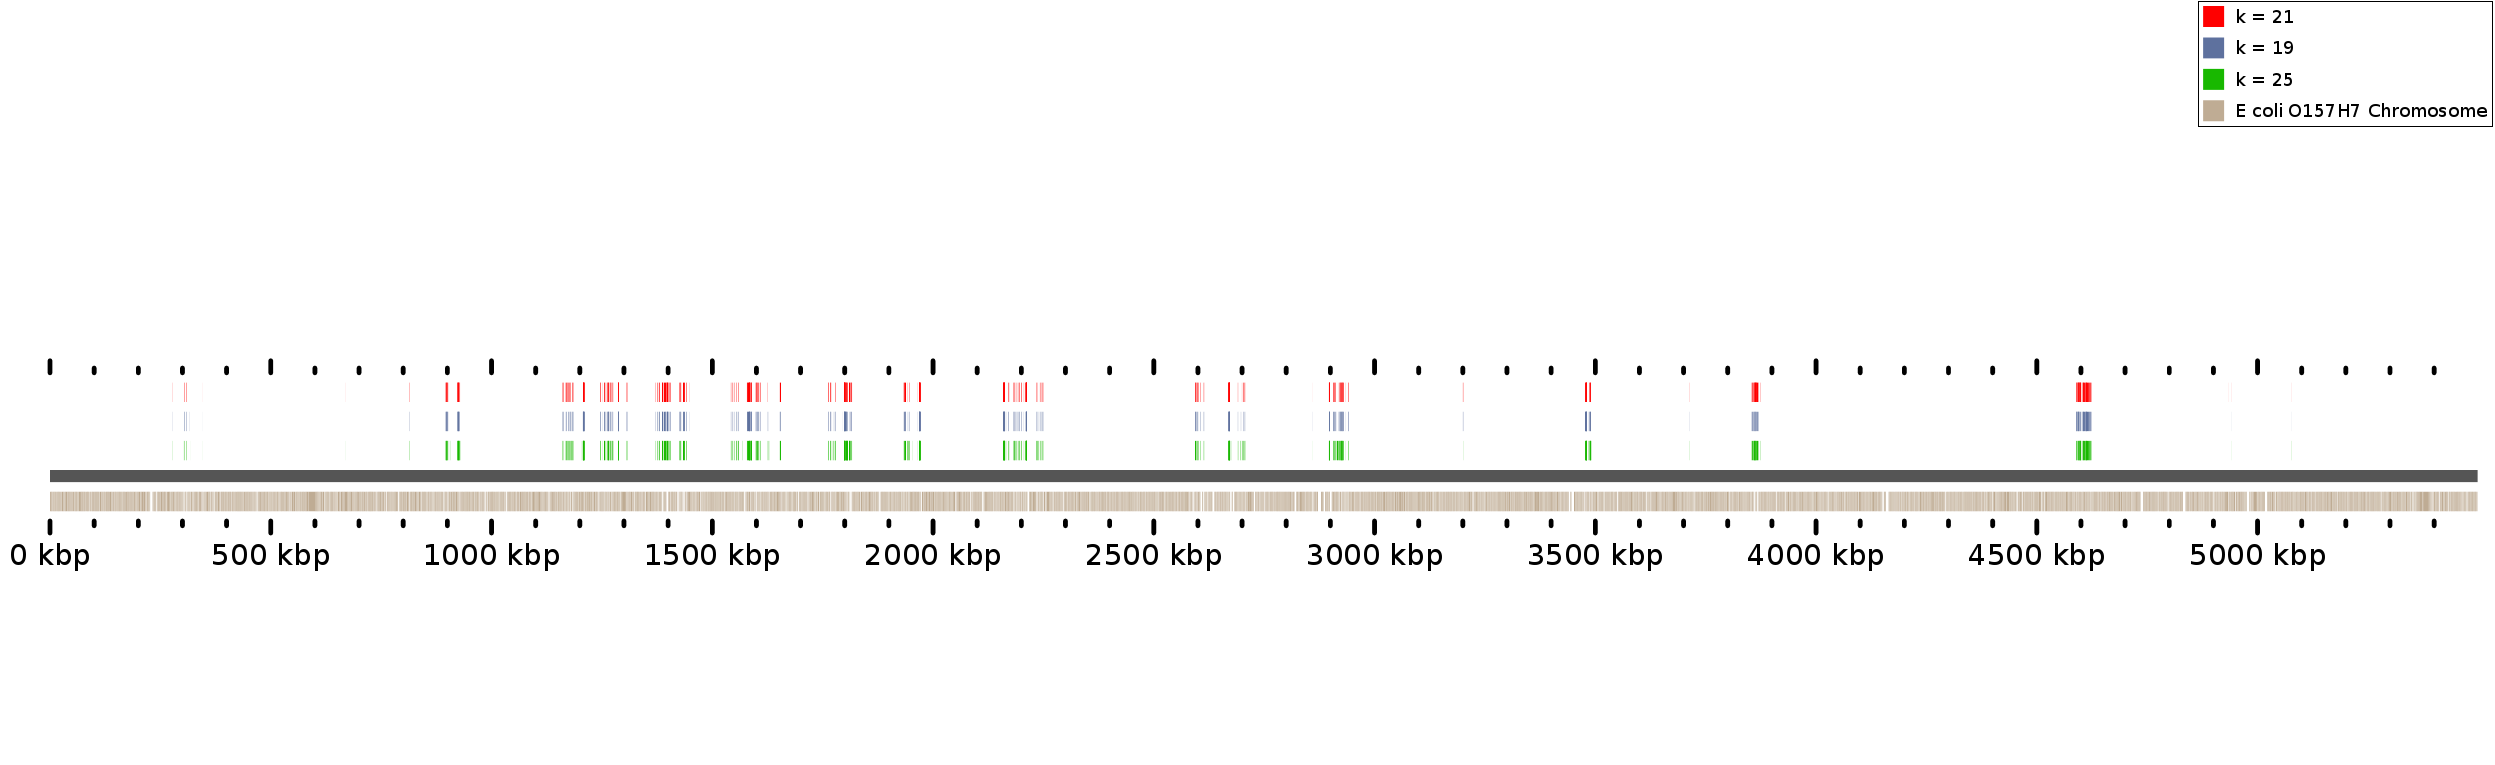
\includegraphics[width=1.0\textwidth]{ecoli_kmers_crop.png}
\caption{A high-level visualization of the signatures identified by Neptune using \textit{k}-mers of different sizes when run on a \textit{E. coli} STEC inclusion and no toxin exclusion dataset. In general, there is considerable agreement about the regions of the genome corresponding to signature sequence.}
\label{figure:ecoli_kmers}
\end{figure}

\end{document}
